% file: SortingPrinciple.tex
% author: C. Menges

\documentclass{standalone}
\usepackage{tikz}
\usetikzlibrary{arrows, calc, arrows.meta}
\begin{document}
	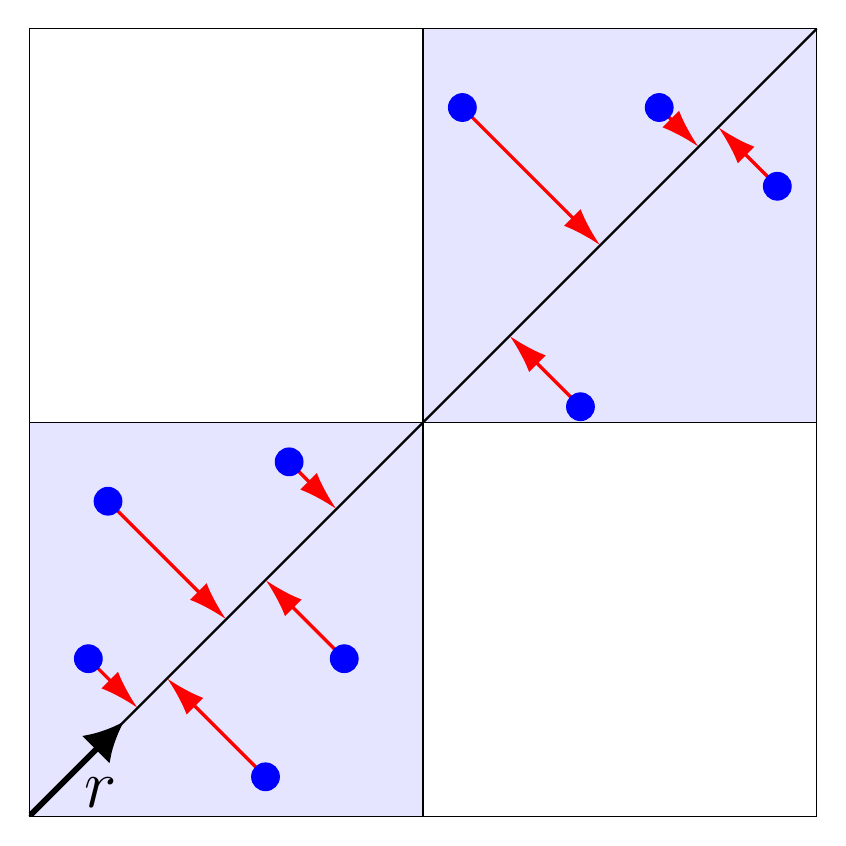
\begin{tikzpicture}
	% interacting cells
	\fill [blue!10] (0,0) rectangle ++(5,5);
	\fill [blue!10] (5,5) rectangle ++(5,5);
	
	% grid
	\draw[step=5.0,black,thin] (0,0) grid (10,10);
	
	% sorting axis
	\draw [thick] (0,0) -- (10,10);
	
	\draw [line width=0.75mm, mark options={scale=10}, -{Latex[length=5mm, width=5mm]}] (0.017,0.017) -> (1.2,1.2);
	\node [] at (0.9,0.3) {\Huge$r$};
	
	%particles
	\def\points{(1,4),(4,2),(3.3,4.5),(0.75,2),(3,0.5),(8,9),(7,5.2),(9.5,8),(5.5,9)}
	
	\foreach \coord [count=\i] in \points {
		\coordinate [at=\coord, name=A\i];
		\draw [very thick, red, mark options={scale=10}, {Latex[length=5mm, width=3mm]}-] ($(0,0)!(A\i)!(10,10)$) -- \coord;
		\filldraw [blue] \coord circle (5pt);
	}
	\end{tikzpicture}
\end{document}